\documentclass{beamer}
\usetheme{Madrid}
\usecolortheme{default}

% Packages
\usepackage{graphicx}
\usepackage{booktabs}
\usepackage{amsmath}
\usepackage{amsfonts}
\usepackage{tabularx}

% Metadata
\title[Cracked Egg Detection via Improved YOLOv8]{\textbf{REAL-TIME DETECTION METHOD FOR CRACKED EGGS BASED ON IMPROVED YOLOV8 AND DUAL VERIFICATION WITH TRIPLE CLASSIFICATION GRANULARITY}}
\subtitle{CSQ413 Seminar Presentation}

\author{
\textbf{Submitted by:} \\ Arjun Manoj (CEC23CS043) \\[0.25cm]
\textbf{Under the Guidance of:} \\ Mrs. NANDANA RAJ R \\ Assistant Professor
}

\institute{
Department of Computer Science and Engineering \\ College of Engineering, Cherthala
}

\date{\today}

\begin{document}

% ==================== TITLE SLIDE ====================
\begin{frame}
  \titlepage
\end{frame}

% ==================== OUTLINE SLIDE ====================
\begin{frame}{Outline}
\tableofcontents
\end{frame}

%=====================================================
\section{Introduction and Problem Statement}
%=====================================================

% ==================== SLIDE 3: INTRODUCTION ====================
\begin{frame}{Introduction: Background and Motivation}
\begin{itemize}
    \item Egg shell integrity is a critical quality indicator in the automated poultry industry.
    \medskip
    \item Approximately 3\% of eggs suffer shell damage during production, handling and transit.
    \medskip
    \item Damaged shells cause bacterial infiltration, accelerate spoilage, lead to yolk leakage and produce heavy economic losses.
    \medskip
    \item Commercial egg inspection in China still primarily relies on manual visual examination:
    \begin{itemize}
        \item High labor intensity and high operating costs.
        \item Low inspection efficiency and strong subjectivity.
        \item Rapid worker fatigue causes elevated error rates and missed detections.
    \end{itemize}
\end{itemize}
\end{frame}

% ==================== SLIDE 4: LIMITATIONS OF EXISTING METHODS ====================
\begin{frame}{Limitations of Existing Methods}
\begin{itemize}
    \item \textbf{Acoustic Resonance Techniques:}
    \begin{itemize}
        \item Analyze resonance frequencies from mechanical tapping response.
        \item Highly sensitive to loud noise in factory environments. High hardware cost.
    \end{itemize}
    \medskip
    \item \textbf{Traditional Computer Vision Approaches:}
    \begin{itemize}
        \item Depend on hand-crafted visual features (Otsu thresholding, morphological operations).
        \item Slow processing speed, weak adaptability and sensitivity to lighting variations.
    \end{itemize}
    \medskip
    \item \textbf{Existing Deep Learning Models:}
    \begin{itemize}
        \item High network complexity and serial processing limit frame rates below production demands ($\ge$ 30 FPS).
        \item Primarily evaluated on static, pre-washed egg images.
        \item Lack rotational conveyor mechanisms, leaving blind spots on the bottom of eggs.
    \end{itemize}
\end{itemize}
\end{frame}

% ==================== SLIDE 5: RESEARCH OBJECTIVES ====================
\begin{frame}{Research Objectives and Key Contributions}
\textbf{Research Objective:} Establish an industrial-grade, real-time online detection method for unwashed cracked eggs on dynamic conveyor lines.

\bigskip
\textbf{Core Contributions of the Study:}
\begin{enumerate}
    \item \textbf{Triple Granularity and Dual Discrimination:}
    Formulated a fine-grained category scheme (intact egg, cracked egg, crack region) and a dual verification rule to prevent missed detections.
    \medskip
    \item \textbf{Structural Optimization of YOLOv8:}
    Integrated DCNv2, BiFPN, WIoUv2 loss function and an extra small object detection head to capture minute, irregular cracks.
    \medskip
    \item \textbf{Industrial Deployment and Validation:}
    Implemented end-to-end online inference on a Kyowa/FP-600 egg conveyor line, achieving 45 FPS and meeting industrial reliability standards.
\end{enumerate}
\end{frame}

%=====================================================
\section{Literature Survey}
%=====================================================

% ==================== SLIDE 6: LITERATURE SURVEY ====================
\begin{frame}{Literature Survey}
\begin{itemize}
    \item \textbf{Traditional and Two-Stage Methods:}
    \begin{itemize}
        \item \textbf{Liang et al. (2020):} Otsu threshold segmentation achieved 98.18\% accuracy, but relied on manual feature extraction and static conditions.
        \item \textbf{Datta et al. (2019):} Faster R-CNN achieved 75\% mAP for severe cracks; heavy two-stage computation was too slow for production lines.
        \item \textbf{Turkoglu (2021):} Hybrid CNN-BiLSTM achieved 96.3\% accuracy, but incurred high computational complexity.
        \item \textbf{Botta et al. (2022):} Deep CNN reached 95.38\% accuracy on static egg images.
    \end{itemize}
    \medskip
    \item \textbf{YOLO Adaptations and Real-Time Systems:}
    \begin{itemize}
        \item \textbf{Yin et al. (2024):} YOLOv5 with Ghost and ECA modules for duck eggs (93.8\% accuracy).
        \item \textbf{Huang et al. (2023):} YOLOv5 with BiFPN and GSConv on unwashed eggs (96.4\% accuracy).
    \end{itemize}
    \medskip
    \item \textbf{Critical Research Gaps Addressed by Base Paper:}
    \begin{itemize}
        \item Non-rotating conveyors fail to inspect bottom cracks.
        \item Binary classification (intact vs cracked) misses subtle micro-cracks under dynamic motion.
    \end{itemize}
\end{itemize}
\end{frame}

%=====================================================
\section{System Hardware and Data Acquisition}
%=====================================================

% ==================== SLIDE 7: MACHINE VISION AND CONVEYOR ====================
\begin{frame}{Machine Vision and Conveying System Setup}
\begin{columns}
    \begin{column}{0.48\textwidth}
        % [FIGURE GUIDANCE]:
        % Place Figure 1 (Egg conveying device) here.
        % File: figure1_egg_conveying_device.jpg
        \begin{figure}[h]
            \centering
            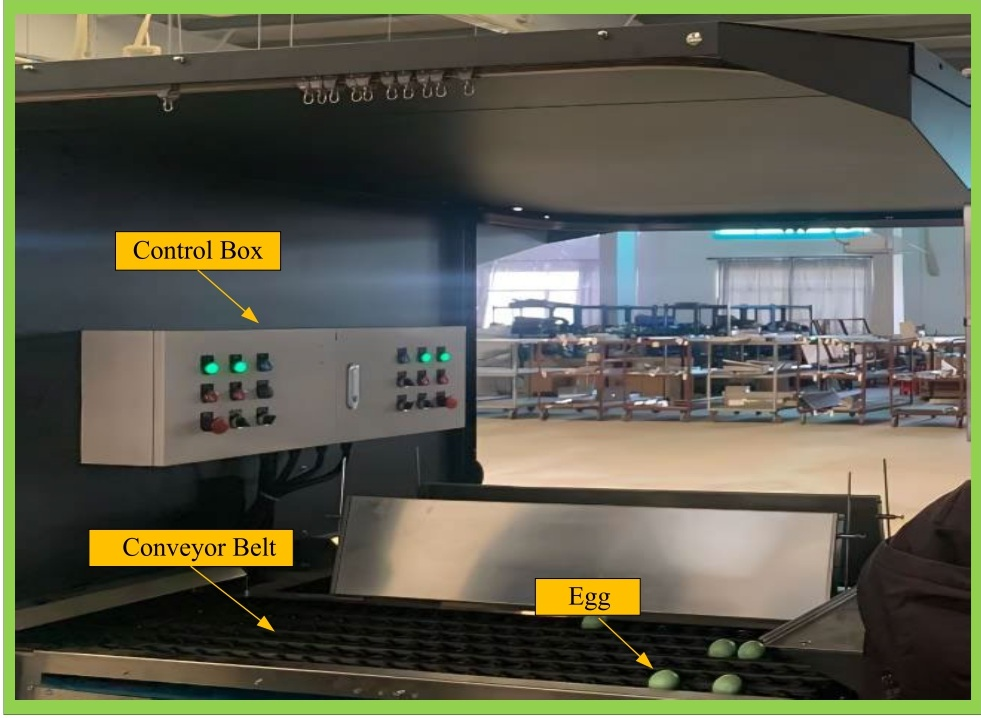
\includegraphics[width=0.8\linewidth,height=0.5\textheight,keepaspectratio]{figure1_egg_conveying_device.jpg}
            \caption{Egg conveying device (Source: Figure 1)}
        \end{figure}
    \end{column}
    \begin{column}{0.52\textwidth}
        % [FIGURE GUIDANCE]:
        % Place Figure 2 (Proposed machine vision system) here.
        % File: figure2_machine_vision_system.jpg
        \begin{figure}[h]
            \centering
            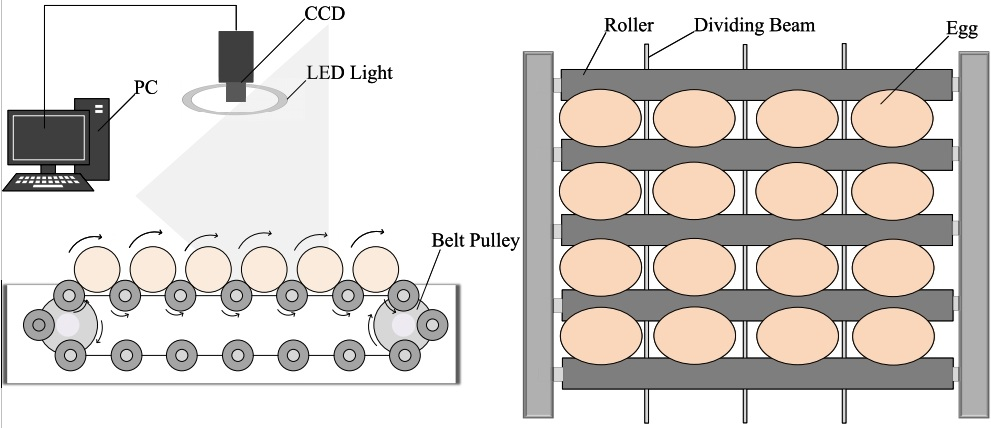
\includegraphics[width=\linewidth]{figure2_machine_vision_system.jpg}
            \caption{Machine vision system layout (Source: Figure 2)}
        \end{figure}
    \end{column}
\end{columns}
\vspace{-0.2cm}
\begin{itemize}
    \item \textbf{Compound Motion:} Six parallel channels (360 eggs/min). Driven rollers rotate eggs 360 degrees, presenting bottom surfaces to the camera.
    \item \textbf{Imaging Rig:} CCD camera plane is parallel to egg motion plane; regulated LED lighting.
\end{itemize}
\end{frame}

% ==================== SLIDE 8: DATASET ACQUISITION AND PREPARATION ====================
\begin{frame}{Dataset Acquisition and Preparation}
\begin{itemize}
    \item \textbf{On-Site Dynamic Image Acquisition:}
    \begin{itemize}
        \item Acquired at Guangzhou Suiping Enterprise Co., Ltd.
        \item Captured unwashed eggs with dust, stains, varying angles and real factory lighting.
        \item Deliberately collected cracked eggs to balance positive and negative samples.
        \item Base raw dataset: 628 dynamic images.
    \end{itemize}
    \medskip
    \item \textbf{Dataset Splitting and Data Augmentation:}
    \begin{itemize}
        \item Split into Training (377), Validation (126) and Test (125) sets in a 6:2:2 ratio.
        \item Applied random cropping and horizontal/vertical flipping (50\% probability) to training set.
        \item Expanded training set to 2,972 images after invalid data removal.
        \item Final dataset: 3,222 images containing 7,611 intact eggs, 2,711 cracked eggs and 2,935 cracked areas.
    \end{itemize}
\end{itemize}
\end{frame}

% ==================== SLIDE 9: TRIPLE GRANULARITY ====================
\begin{frame}{Triple Classification Granularity and Annotation}
\begin{itemize}
    \item \textbf{Limitation of Binary Classification:}
    \begin{itemize}
        \item Binary labels ("intact" vs "cracked") force the model to rely only on whole-egg features.
        \item Small local cracks contribute minor global visual cues, causing high false negatives.
    \end{itemize}
    \medskip
    \item \textbf{Proposed Triple Classification Scheme:}
    \begin{itemize}
        \item \textbf{Category 1 (Intact Egg):} Normal undamaged egg body.
        \item \textbf{Category 2 (Cracked Egg):} Entire egg body displaying cracks.
        \item \textbf{Category 3 (Crack Region):} Specific localized damaged fracture zone.
    \end{itemize}
    \medskip
    \item \textbf{Annotation Protocol:}
    \begin{itemize}
        \item Annotated using LabelImg with labels "1", "2" and "3".
        \item XML annotations converted to YOLO-compatible TXT format.
        \item Enriches feature representations with both macro-level and micro-level cues.
    \end{itemize}
\end{itemize}
\end{frame}

%=====================================================
\section{Proposed Improved YOLOv8 Methodology}
%=====================================================

% ==================== SLIDE 10: ARCHITECTURE OVERVIEW ====================
\begin{frame}{Improved YOLOv8 Network Architecture Overview}
% [FIGURE GUIDANCE]:
% Figure 3 split into two horizontal parts for enhanced legibility.
% Part 1: Main improved YOLOv8 detection architecture (Backbone, BiFPN neck, 4 Detect heads).
% Part 2: Detailed sub-module blocks (C2f_1, C2f_2, BottleNeck, SPPF).
\begin{figure}[h]
    \centering
    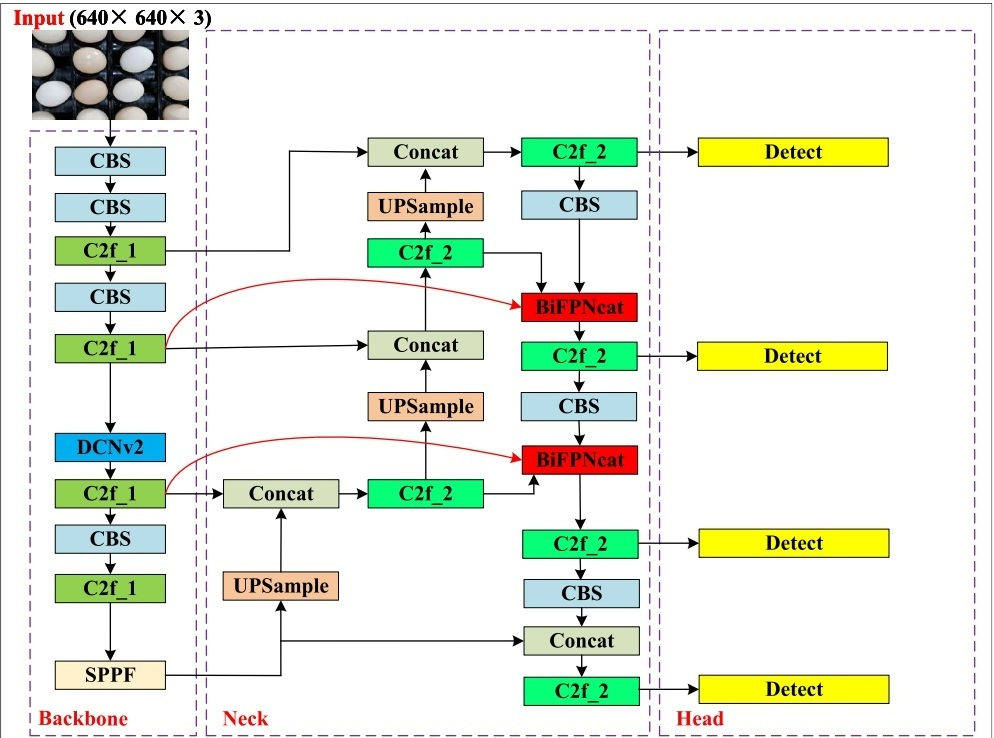
\includegraphics[width=0.5\linewidth,height=0.42\textheight, keepaspectratio]{figure3_improved_yolov8_architecture_1.jpg}
    \hfill
    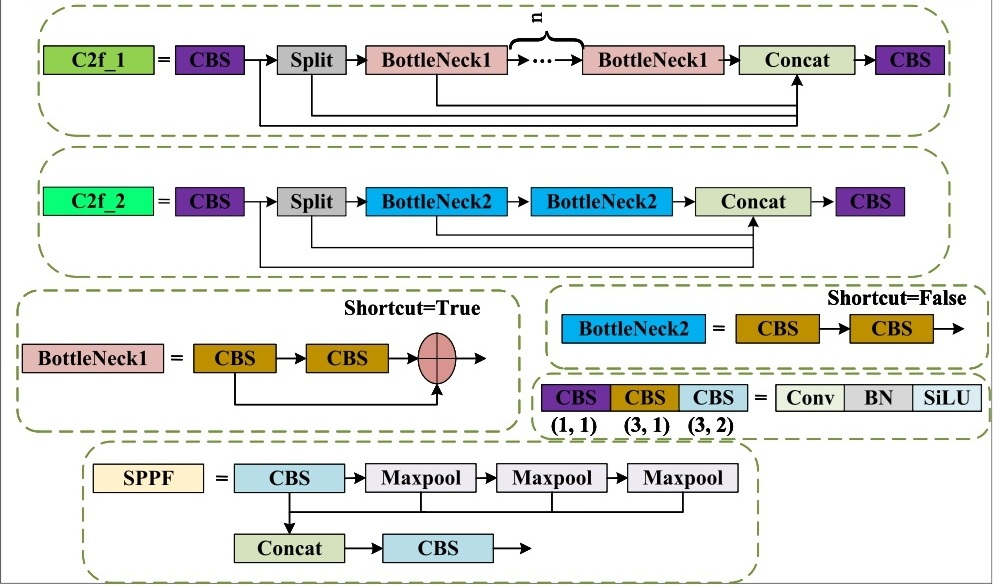
\includegraphics[width=0.48\linewidth,height=0.42\textheight, keepaspectratio]{figure3_improved_yolov8_architecture_2.jpg}
    \vspace{-0.2cm}
    \caption{\scriptsize Architecture of the proposed improved YOLOv8 model (Source: Base Paper Figure 3)}
    \end{figure}
    \vspace{-0.2cm}
    \begin{itemize}
        \item Retains anchor-free split Ultralytics head for optimal accuracy-speed trade-off.
        \item Integrates four dedicated innovations: DCNv2, BiFPN, Small Object Head and WIoUv2.
\end{itemize}
\end{frame}

% ==================== SLIDE 11: DCNv2 ====================
\begin{frame}{Architectural Enhancement 1: Deformable Convolutions (DCNv2)}
\begin{columns}[t]
    \begin{column}{0.54\textwidth}
        \small
        \textbf{Limitation of Standard Convolutions:}
        \begin{itemize}
            \item Rigid square sampling grids cannot adapt to irregular, jagged crack contours.
        \end{itemize}
        \smallskip
        \textbf{DCNv2 Formulation:}
        \vspace{-0.15cm}
        \begin{equation*}
        \small Y(q) = \sum_{k=1}^{K} w_k X(q + q_k + \Delta q_k) \Delta m_k
        \end{equation*}
        \vspace{-0.25cm}
        \begin{itemize}
            \item $\Delta q_k$: Learnable 2D spatial offset matching crack geometry.
            \item $\Delta m_k \in [0, 1]$: Dynamic modulation scalar scaling feature amplitude.
            \item Amplifies crack features while suppressing background shell noise.
        \end{itemize}
    \end{column}
    \begin{column}{0.46\textwidth}
        % [FIGURE GUIDANCE]:
        % Place Figure 4 (Comparison of DNv1, DCNv2 and Normal Conv sampling) here.
        % File: figure4_dcnv2_sampling_comparison.jpg
        \begin{figure}[h]
            \centering
            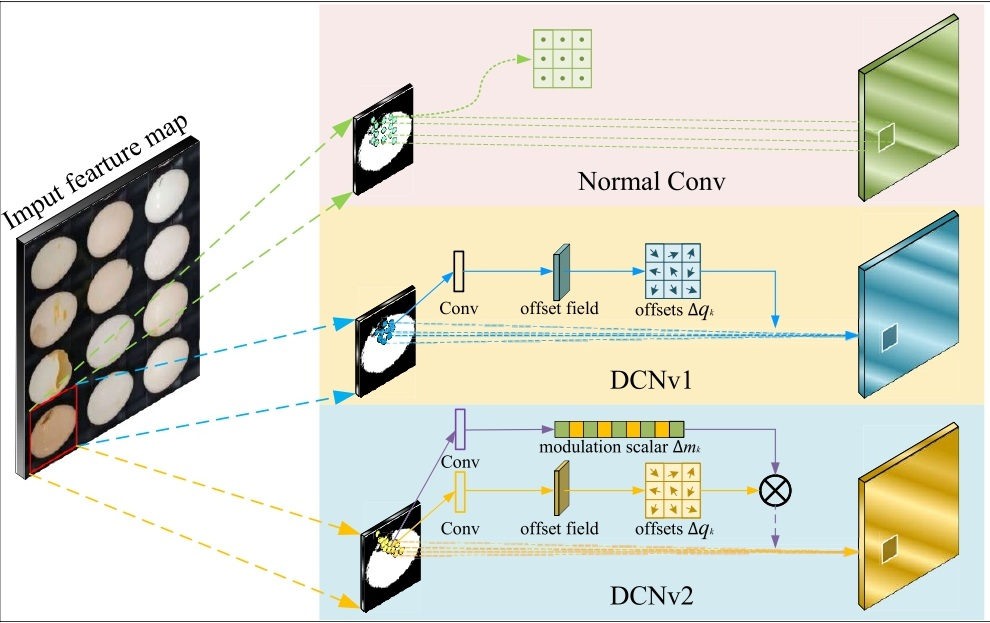
\includegraphics[width=\linewidth,height=0.52\textheight, keepaspectratio]{figure4_dcnv2_sampling_comparison.jpg}
            \vspace{-0.2cm}
            \caption{\scriptsize Sampling comparison: Normal Conv, DCNv1, DCNv2 (Source: Figure 4)}
        \end{figure}
    \end{column}
\end{columns}
\end{frame}

% ==================== SLIDE 12: BiFPN ====================
\begin{frame}{Architectural Enhancement 2: BiFPN Multi-Scale Fusion}
\begin{columns}
    \begin{column}{0.52\textwidth}
        \textbf{From FPN and PANet to BiFPN:}
        \begin{itemize}
            \item \textbf{FPN:} Top-down path for semantic feature integration.
            \item \textbf{PANet (Default YOLOv8):} Added bottom-up path for low-level spatial features.
            \item \textbf{BiFPN:} Removes single-edge nodes, adds cross-scale skip connections and repeats blocks.
        \end{itemize}
        \medskip
        \textbf{Key Benefits for Crack Inspection:}
        \begin{itemize}
            \item Dynamically weights feature maps based on contribution.
            \item Maintains strong representation under lighting variations and dirty shell backgrounds.
        \end{itemize}
    \end{column}
    \begin{column}{0.48\textwidth}
        % [FIGURE GUIDANCE]:
        % Place Figure 5 (The structure of FPN, PANet and BiFPN) here.
        % File: figure5_fpn_panet_bifpn_structure.jpg
        \begin{figure}[h]
            \centering
            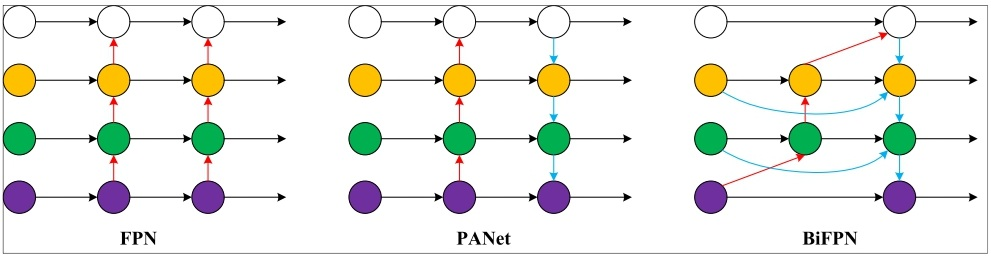
\includegraphics[width=\linewidth]{figure5_fpn_panet_bifpn_structure.jpg}
            \caption{Architectural comparison of FPN, PANet and BiFPN (Source: Base Paper Figure 5)}
        \end{figure}
    \end{column}
\end{columns}
\end{frame}

% ==================== SLIDE 13: SMALL OBJECT HEAD AND WIoUv2 ====================
\begin{frame}{Enhancements 3 \& 4: Small Target Head and WIoUv2 Loss}
\begin{itemize}
    \item \textbf{Enhancement 3: Dedicated Small Object Detection Layer}
    \begin{itemize}
        \item Standard YOLOv8 5 downsamplings ($/32$) yield an $80 \times 80$ head with receptive field $8 \times 8$ px; micro-cracks under 8 px vanish in deep layers.
        \item Integrated a 4th detection head operating on a $160 \times 160$ feature map (P2 layer).
        \item Directly captures fine spatial textures and edge gradients from earlier stages.
    \end{itemize}
    \medskip
    \item \textbf{Enhancement 4: Wise-IoU v2 (WIoUv2) Loss Function}
    \begin{equation*}
    L_{\text{WIoUv2}} = L_{\text{IoU}}^{\gamma*} L_{\text{WIoUv1}}, \quad \gamma > 0
    \end{equation*}
    \begin{itemize}
        \item Standard CIoU ignores sample quality variations during dynamic conveyor motion.
        \item Dynamic focusing factor $L_{\text{IoU}}^{\gamma*}$ adaptively balances gradient contributions.
        \item Handles class imbalance and enhances detection of occluded or motion-blurred cracks.
    \end{itemize}
\end{itemize}
\end{frame}

% ==================== SLIDE 14: DUAL VERIFICATION MECHANISM ====================
\begin{frame}{Dual Verification Decision-Making Mechanism}
\begin{itemize}
    \item \textbf{Post-Processing Decision Rule:}
    \begin{itemize}
        \item Standard sorting systems decide based only on whole-egg bounding boxes.
        \item Under the proposed rule, an egg is tagged as \textbf{damaged} if the detector outputs:
        \begin{center}
            \textbf{Category 2 (Cracked Egg)} \quad \textit{OR} \quad \textbf{Category 3 (Crack Region)}
        \end{center}
    \end{itemize}
    \medskip
    \item \textbf{Mathematical Joint Miss Rate Reduction:}
    \begin{itemize}
        \item A damaged egg is missed \textbf{only if both} Category 2 and Category 3 fail simultaneously:
        \begin{equation*}
        P(\text{Miss}_{\text{Overall}}) = P(\text{Miss}_{\text{Egg}}) \times P(\text{Miss}_{\text{Region}})
        \end{equation*}
        \item Global shape cues and local fracture cues cross-verify each other.
        \item Lowers industrial false negative rates while preventing unnecessary waste.
    \end{itemize}
\end{itemize}
\end{frame}

%=====================================================
\section{Experimental Setup and Evaluation}
%=====================================================

% ==================== SLIDE 15: EXPERIMENTAL ENVIRONMENT ====================
\begin{frame}{Experimental Platform and Training Setup}
\begin{columns}
    \begin{column}{0.54\textwidth}
        \textbf{Hardware and Software Specifications:}
        \begin{itemize}
            \item \textbf{Operating System:} Windows 10
            \item \textbf{Framework:} Python 3.8, PyTorch 1.13.1, CUDA 11.6
            \item \textbf{Processor:} Intel Core i5-10400F @ 2.9 GHz
            \item \textbf{Graphics Card:} NVIDIA GeForce RTX 3060 (12 GB VRAM)
            \item \textbf{System Memory:} 32 GB DDR4 (3200 MHz)
        \end{itemize}
        \medskip
        \textbf{Hyperparameters:}
        \begin{itemize}
            \item Input resolution: $640 \times 640$ pixels
            \item Epochs: 300 iterations; Batch size: 16
            \item Initial learning rate: 0.01; Seed: 42
            \item Trained strictly from scratch (no pre-trained weights).
        \end{itemize}
    \end{column}
    \begin{column}{0.46\textwidth}
        % [FIGURE GUIDANCE]:
        % Place Figure 6 (Training schematic of the cracked eggs detection model) here.
        % File: figure6_training_schematic.jpg
        \begin{figure}[h]
            \centering
            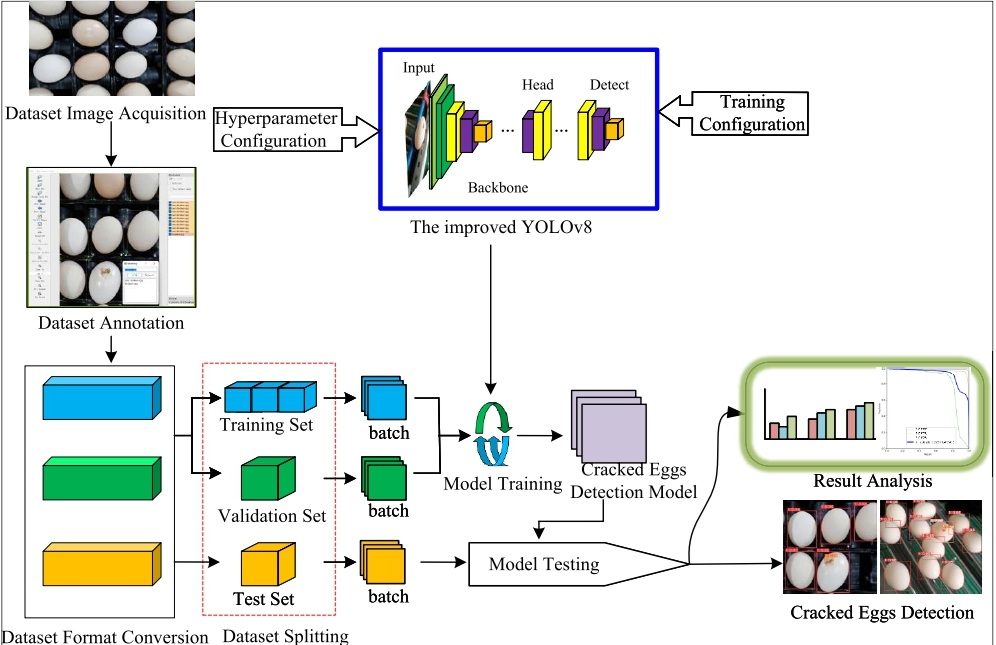
\includegraphics[width=\linewidth]{figure6_training_schematic.jpg}
            \caption{Training and validation workflow (Source: Base Paper Figure 6)}
        \end{figure}
    \end{column}
\end{columns}
\end{frame}

% ==================== SLIDE 16: EVALUATION METRICS ====================
\begin{frame}{Evaluation Metrics}
\begin{itemize}
    \item \textbf{Precision (P):} Proportion of detected cracked items that are truly cracked:
    \begin{equation*}
    \text{Precision} = \frac{\text{TP}}{\text{TP} + \text{FP}}
    \end{equation*}
    \item \textbf{Recall (R):} Proportion of actual cracked items correctly detected:
    \begin{equation*}
    \text{Recall} = \frac{\text{TP}}{\text{TP} + \text{FN}}
    \end{equation*}
    \item \textbf{Mean Average Precision (mAP@0.5):} Comprehensive accuracy score computed as the area under the PR curve across all categories.
    \medskip
    \item \textbf{Frames Per Second (FPS):} Real-time processing speed ($\ge 30$ FPS needed on lines).
    \medskip
    \item \textbf{Industrial Reliability Metrics:}
    \begin{itemize}
        \item \textbf{False Negative Rate (FNR):} Ratio of missed damaged eggs (product safety).
        \item \textbf{False Positive Rate (FPR):} Ratio of good eggs falsely rejected (waste control).
    \end{itemize}
\end{itemize}
\end{frame}

%=====================================================
\section{Results and Performance Analysis}
%=====================================================

% ==================== SLIDE 17: ABLATION STUDY AND COMPLEXITY ====================
\begin{frame}{Ablation Study and Model Complexity}
\begin{table}[h]
\centering
\caption{\scriptsize Ablation experiment results on test dataset (Source: Base Paper Table 1)}
\vspace{-0.3cm}
\setlength{\tabcolsep}{3pt}
\renewcommand{\arraystretch}{0.92}
\resizebox{0.95\textwidth}{!}{
\begin{tabular}{cccc|ccc}
\toprule
\textbf{DCNv2} & \textbf{BiFPN} & \textbf{WIoU} & \textbf{Small Target} & \textbf{Precision (\%)} & \textbf{Recall (\%)} & \textbf{mAP:0.5 (\%)} \\
\midrule
- & - & - & - & 92.2 & 85.3 & 87.7 \\
- & - & \checkmark & - & 90.6 & 87.4 & 90.3 \\
- & \checkmark & - & - & 89.8 & 83.8 & 88.2 \\
- & - & - & \checkmark & 93.8 & 90.3 & 93.0 \\
\checkmark & - & \checkmark & - & 93.1 & 89.4 & 92.1 \\
- & \checkmark & \checkmark & - & 92.6 & 89.5 & 92.2 \\
\checkmark & \checkmark & \checkmark & - & 93.8 & 89.9 & 92.6 \\
\checkmark & \checkmark & \checkmark & \checkmark & \textbf{94.1} & \textbf{90.0} & \textbf{92.9} \\
\bottomrule
\end{tabular}
}
\end{table}
\vspace{-0.35cm}
{\small
\begin{itemize}
    \setlength{\itemsep}{1pt}
    \item Small target head yields the largest single mAP gain (+5.3\%). Full ensemble achieves the highest overall Precision (94.1\%) and balanced robustness.
    \item \textbf{Model Complexity (Table 2):} Parameters: $2.66 \times 10^7$ (+2.7\%), FLOPs: 86.5 G (+9.3\%), Model Size: 51.1 MB (+3.0\%). Significant accuracy boost achieved with minimal overhead.
\end{itemize}
}
\end{frame}

% ==================== SLIDE 18: BENCHMARK COMPARISON ====================
\begin{frame}{Comparative Experiments with Mainstream Detectors}
\begin{table}[h]
\centering
\caption{\scriptsize Comparison across different object detection models (Source: Base Paper Table 3)}
\vspace{-0.3cm}
\setlength{\tabcolsep}{5pt}
\renewcommand{\arraystretch}{0.95}
\resizebox{0.92\textwidth}{!}{
\begin{tabular}{lcccc}
\toprule
\textbf{Model} & \textbf{Precision (\%)} & \textbf{Recall (\%)} & \textbf{mAP:0.5 (\%)} & \textbf{FPS} \\
\midrule
Faster R-CNN (ResNet50) & 68.4 & 80.7 & 78.1 & 17 \\
YOLOv5 & 86.9 & 81.1 & 85.2 & 58 \\
YOLOv8 (Baseline) & 92.2 & 85.3 & 87.7 & 52 \\
YOLOv11 & 92.7 & 84.3 & 87.3 & 47 \\
\textbf{Our Proposed Model} & \textbf{94.1} & \textbf{90.0} & \textbf{92.9} & \textbf{45} \\
\bottomrule
\end{tabular}
}
\end{table}
\vspace{-0.25cm}
{\small
\begin{itemize}
    \setlength{\itemsep}{2pt}
    \item Outperformed Faster R-CNN by 14.8\% mAP despite Faster R-CNN using pretrained weights while our model trained from scratch.
    \item Outperformed recent YOLOv11 by 5.6\% mAP and baseline YOLOv8 by 5.2\% mAP.
    \item At 45 FPS, detection speed easily satisfies the production requirement ($\ge 30$ FPS).
\end{itemize}
}
\end{frame}

% ==================== SLIDE 19: QUALITATIVE LABORATORY DETECTION ====================
\begin{frame}{Laboratory Simulated Platform Testing}
\begin{columns}[t]
    \begin{column}{0.5\textwidth}
        % [FIGURE GUIDANCE]:
        % Place Figure 8 (The accuracy of online detection before and after model improvement) here.
        % File: figure8_pr_curves_comparison.jpg
        \begin{figure}[h]
            \centering
            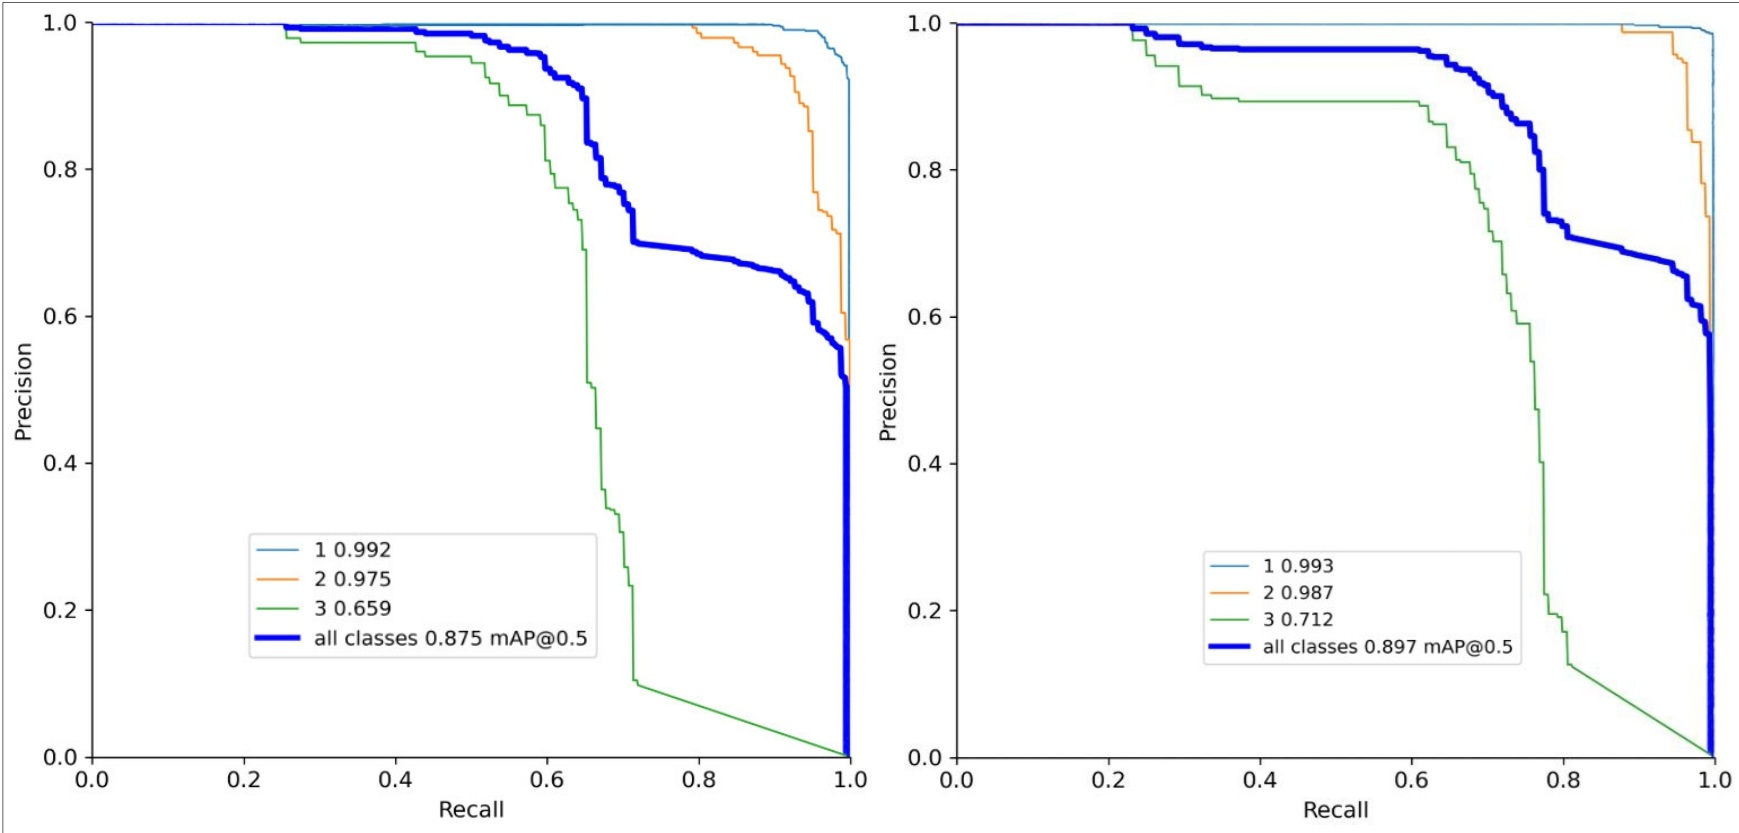
\includegraphics[width=\linewidth,height=0.45\textheight,keepaspectratio]{figure8_pr_curves_comparison.jpg}
            \vspace{-0.2cm}
            \caption{\scriptsize PR curves comparison (Source: Figure 8)}
        \end{figure}
    \end{column}
    \begin{column}{0.5\textwidth}
        % [FIGURE GUIDANCE]:
        % Place Figure 9 (Comparison of online detection effects before and after model improvement) here.
        % File: figure9_detection_effects_comparison.jpg
        \begin{figure}[h]
            \centering
            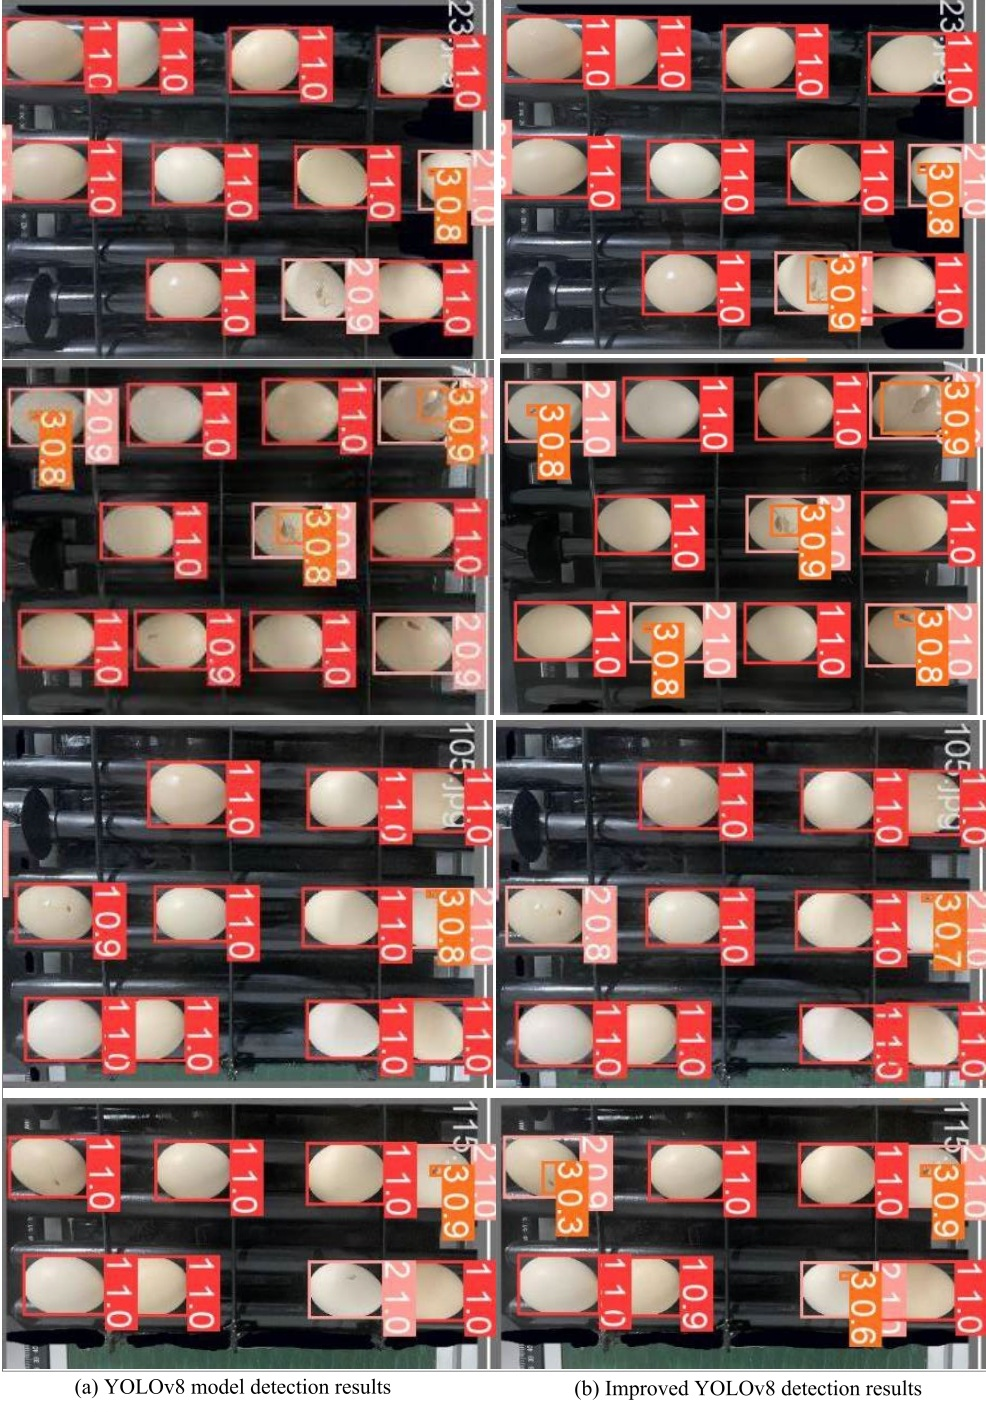
\includegraphics[width=\linewidth,height=0.45\textheight,keepaspectratio]{figure9_detection_effects_comparison.jpg}
            \vspace{-0.2cm}
            \caption{\scriptsize Visual detection comparison (Source: Figure 9)}
        \end{figure}
    \end{column}
\end{columns}
\vspace{-0.25cm}
{\small
\begin{itemize}
    \setlength{\itemsep}{1pt}
    \item Tested on 115 video frames: improved model achieves 2.5\% higher mAP.
    \item Successfully identifies micro-cracks where original YOLOv8 produced missed detections.
\end{itemize}
}
\end{frame}

% ==================== SLIDE 20: FACTORY TESTING SETUP ====================
\begin{frame}{Industrial Deployment on Factory Equipment}
\begin{columns}[t]
    \begin{column}{0.52\textwidth}
        \small
        \textbf{On-Site Equipment (Kyowa/FP-600 Line):}
        \begin{itemize}
            \setlength{\itemsep}{1pt}
            \item Conveyor velocity: 0.1 m/s.
            \item Camera: A3200CU000 ($1920 \times 1080$) at 120 FPS.
            \item Host CPU: 12th Gen Intel i5-12400F (2.50 GHz).
            \item Host GPU: GeForce RTX 3060 Ti 8G; 16 GB RAM.
            \item Environment: Python 3.8, PyTorch 1.13.1, CUDA 11.6.
        \end{itemize}
        \smallskip
        \textbf{Operational Speed:}
        \begin{itemize}
            \item Original YOLOv8: 52 FPS.
            \item Proposed Model: 45 FPS (fully real-time).
        \end{itemize}
    \end{column}
    \begin{column}{0.48\textwidth}
        % [FIGURE GUIDANCE]:
        % Figure 7 split into two stacked parts for clear visualization.
        % Part 1: figure7_online_deployment_testing_1.jpg (874 x 1009)
        % Part 2: figure7_online_deployment_testing_2.jpg (1150 x 1009)
        \begin{figure}[h]
            \centering
            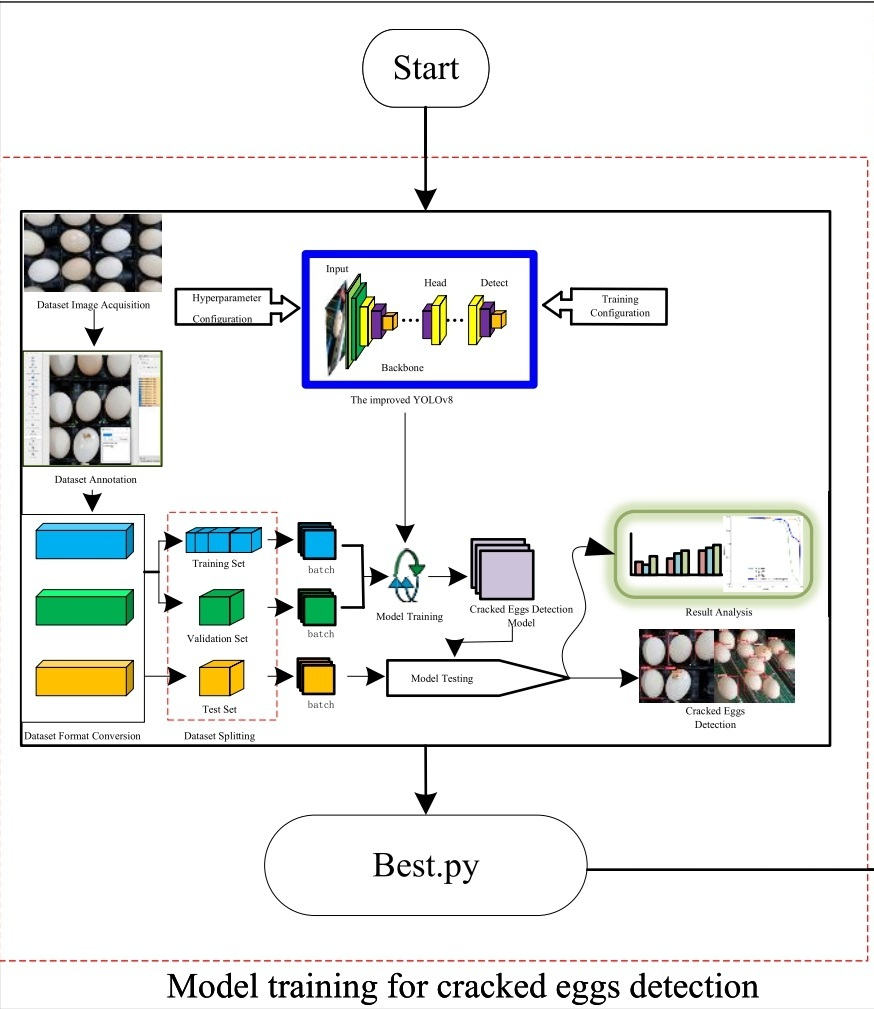
\includegraphics[width=0.88\linewidth,height=0.32\textheight,keepaspectratio]{figure7_online_deployment_testing_1.jpg} \\
            \vspace{0.1cm}
            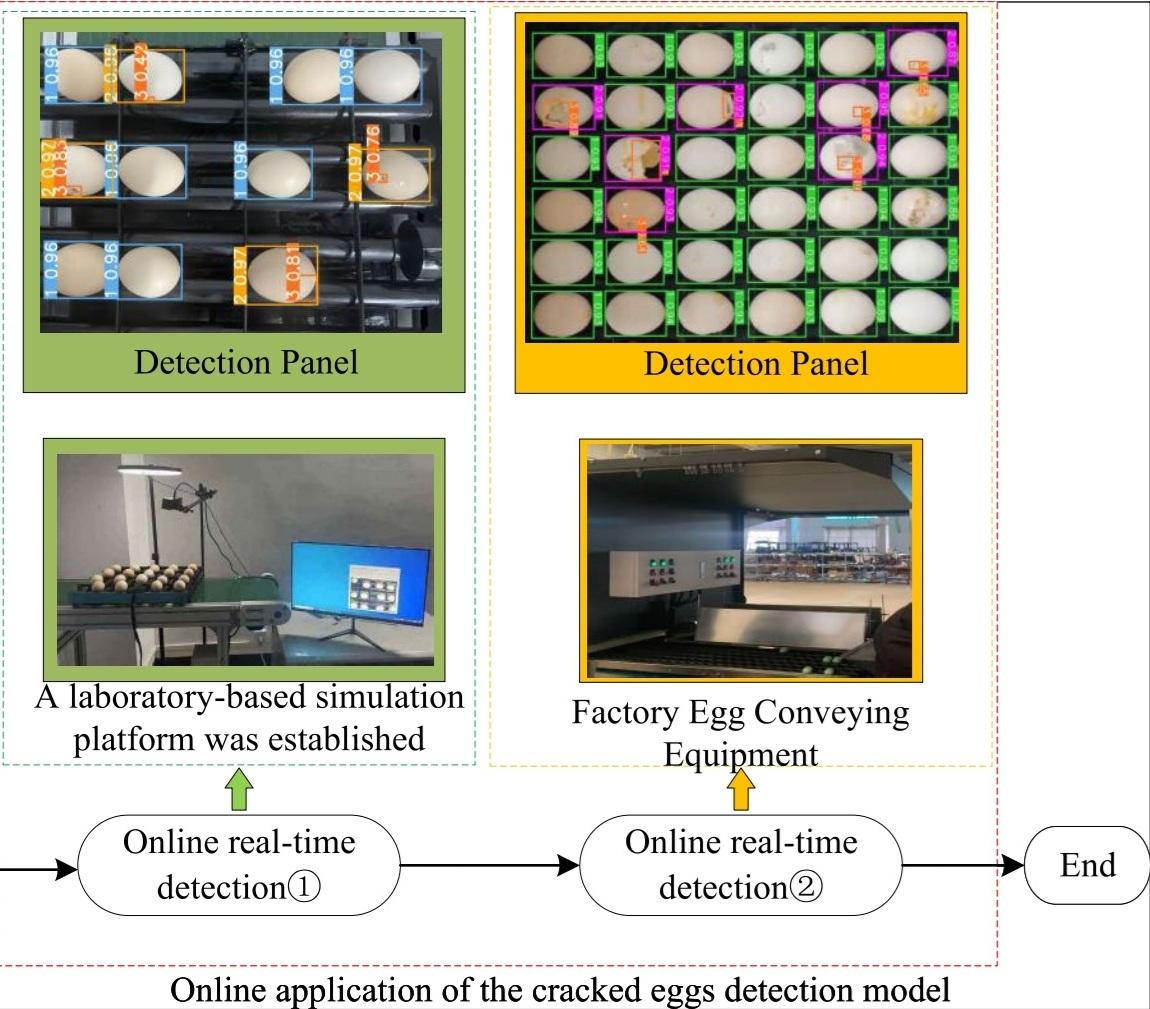
\includegraphics[width=0.88\linewidth,height=0.32\textheight,keepaspectratio]{figure7_online_deployment_testing_2.jpg}
            \vspace{-0.2cm}
            \caption{\scriptsize Online deployment on factory equipment (Source: Figure 7)}
        \end{figure}
    \end{column}
\end{columns}
\end{frame}

% ==================== SLIDE 21: INDUSTRIAL RELIABILITY ANALYSIS ====================
\begin{frame}{Factory Online Inspection Accuracy (FNR and FPR)}
\begin{table}[h]
\centering
\caption{\scriptsize Online inspection comparison on 106 production frames (Source: Base Paper Tables 5 and 6)}
\vspace{-0.3cm}
\setlength{\tabcolsep}{3.5pt}
\renewcommand{\arraystretch}{0.92}
\resizebox{0.95\textwidth}{!}{
\begin{tabular}{l|cc|cc}
\toprule
\textbf{Category} & \multicolumn{2}{c|}{\textbf{Baseline YOLOv8}} & \multicolumn{2}{c}{\textbf{Proposed Improved YOLOv8}} \\
& \textbf{FNR (\%)} & \textbf{FPR (\%)} & \textbf{FNR (\%)} & \textbf{FPR (\%)} \\
\midrule
Class 1: Intact Egg & 1.26 & 4.00 & \textbf{0.46} & \textbf{2.18} \\
Class 2: Cracked Egg & 10.17 & 3.20 & \textbf{5.52} & \textbf{1.16} \\
Class 3: Damaged Area & 22.97 & 0.87 & \textbf{19.19} & \textbf{0.58} \\
\midrule
\textbf{Compound Dual Verification FNR} & \multicolumn{2}{c|}{$10.17\% \times 22.97\% = 2.34\%$} & \multicolumn{2}{c}{$\mathbf{5.52\% \times 19.19\% = 1.06\%}$} \\
\bottomrule
\end{tabular}
}
\end{table}
\vspace{-0.3cm}
{\small
\begin{itemize}
    \setlength{\itemsep}{1pt}
    \item False alarm rate for intact eggs dropped from 4.00\% to 2.18\%, saving intact eggs.
    \item Compound miss rate for cracked eggs fell to 1.06\%, reliably filtering defective eggs.
\end{itemize}
}
\end{frame}

% ==================== SLIDE 22: VISUAL PRODUCTION LINE DETECTIONS ====================
\begin{frame}{Production Line Visual Detections and Speed Stability}
\begin{columns}
    \begin{column}{0.5\textwidth}
        % [FIGURE GUIDANCE]:
        % Place Figure 10 (Detection effect on the actual production line) here.
        % File: figure10_production_line_detection.jpg
        \begin{figure}[h]
            \centering
            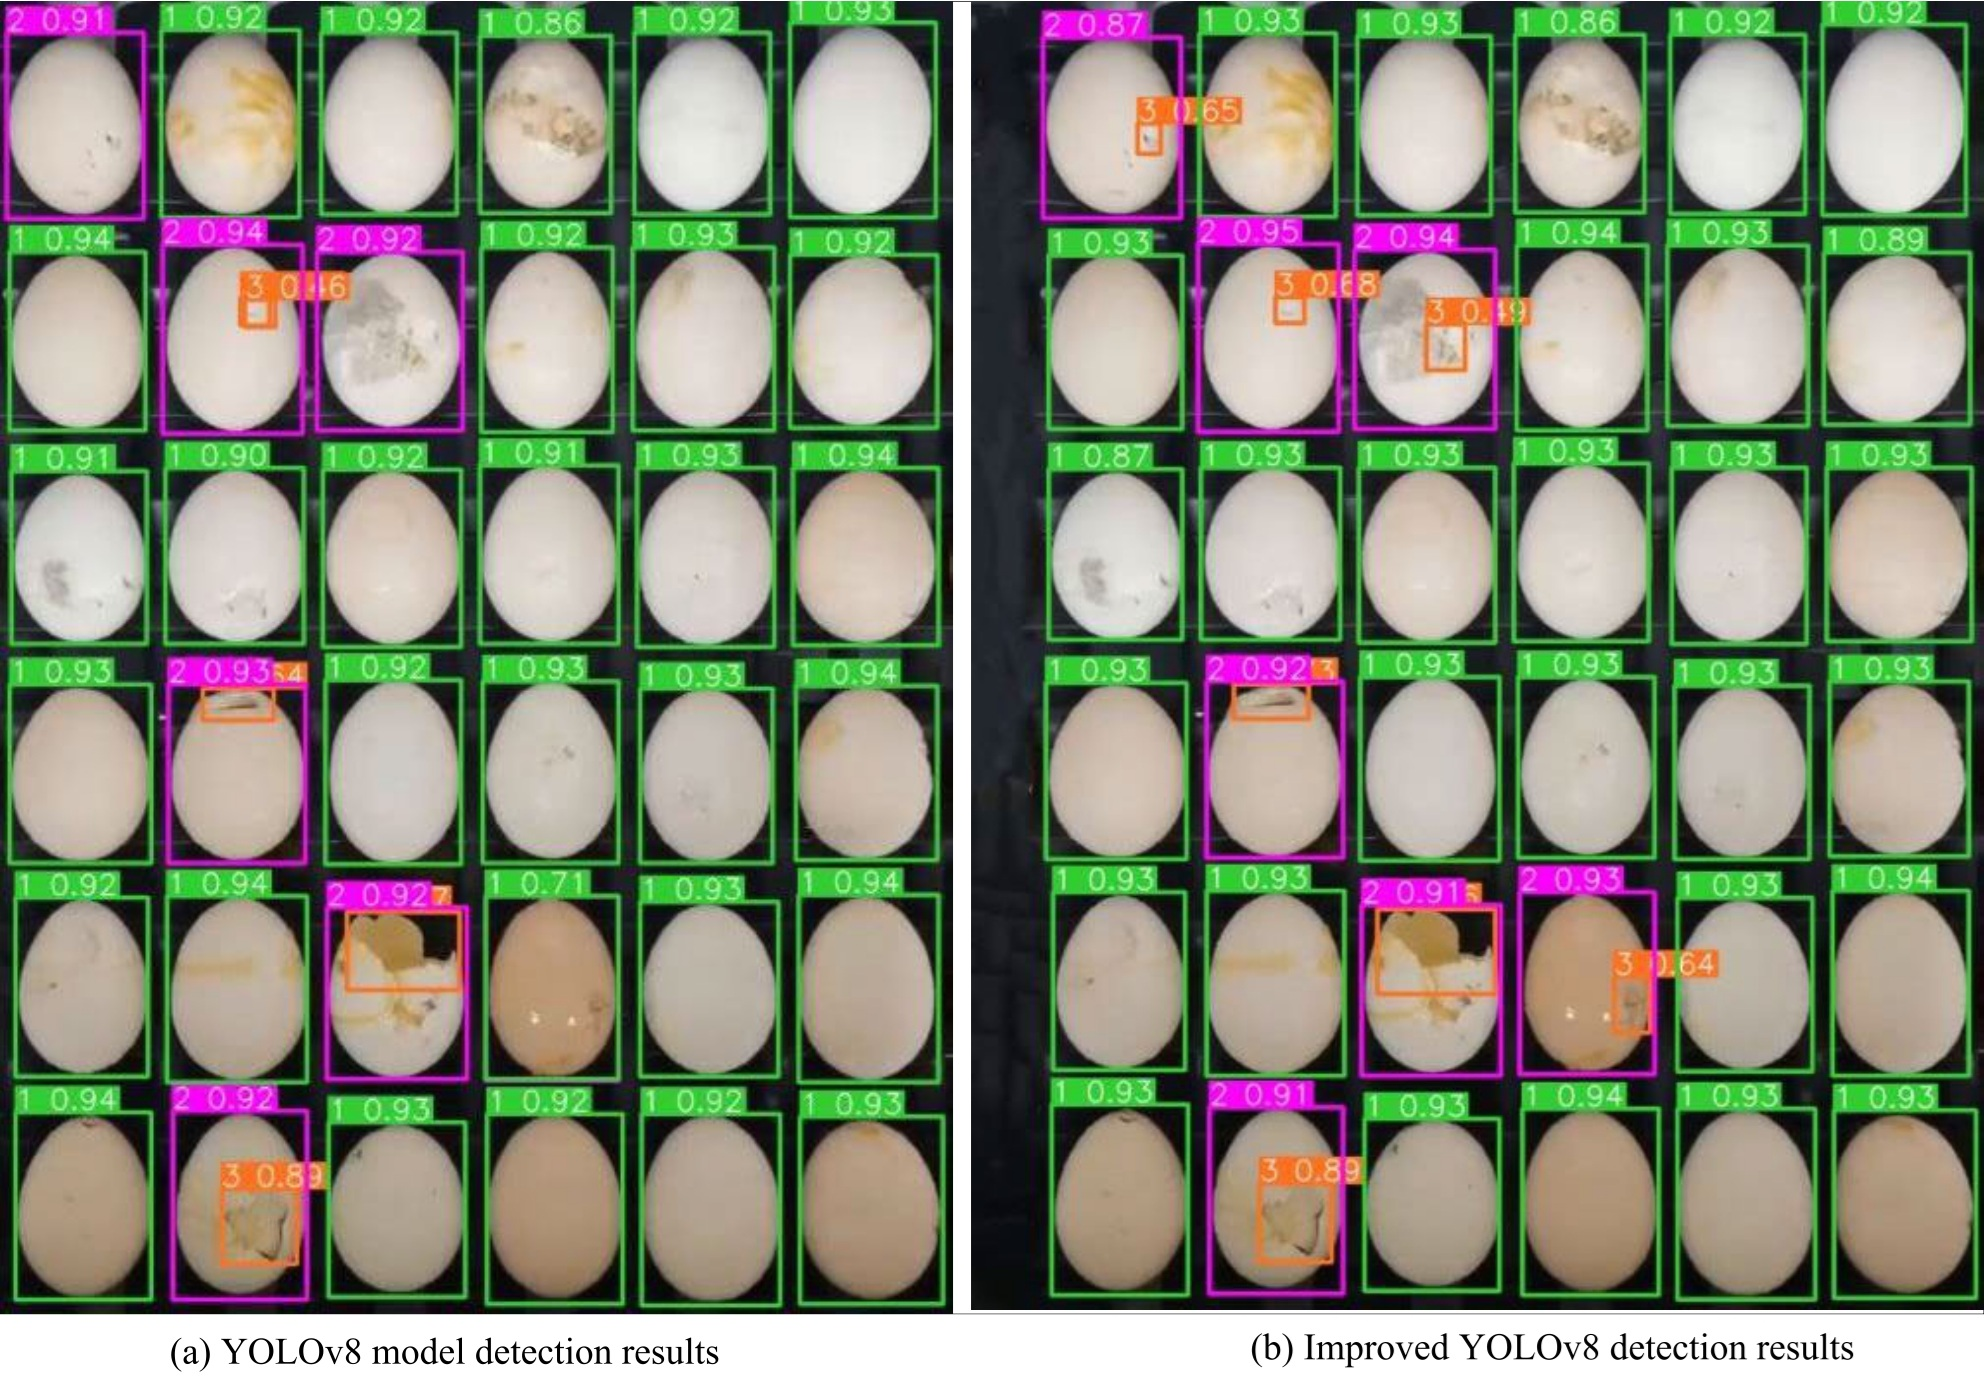
\includegraphics[width=\linewidth]{figure10_production_line_detection.jpg}
            \caption{Detection on actual production line (Source: Figure 10)}
        \end{figure}
    \end{column}
    \begin{column}{0.5\textwidth}
        % [FIGURE GUIDANCE]:
        % Place Figure 11 (Speed of online detection before and after model improvement) here.
        % File: figure11_online_detection_speed.jpg
        \begin{figure}[h]
            \centering
            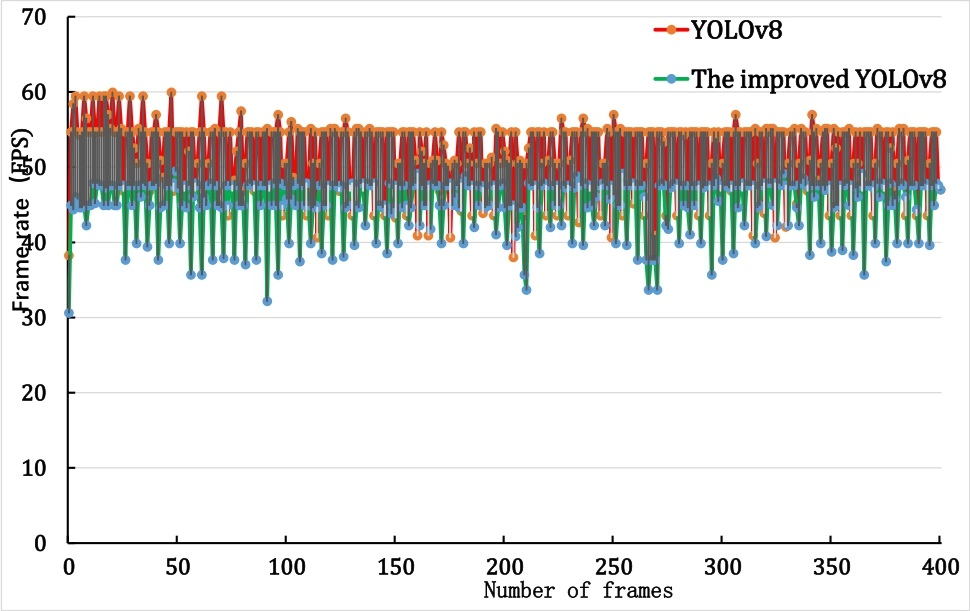
\includegraphics[width=\linewidth]{figure11_online_detection_speed.jpg}
            \caption{Speed stability across 400 frames (Source: Figure 11)}
        \end{figure}
    \end{column}
\end{columns}
\begin{itemize}
    \item Stable inference performance across continuous 400-frame video testing.
    \item Accurately detects cracked eggs and damaged areas under variable industrial lighting.
\end{itemize}
\end{frame}

%=====================================================
\section{Discussion and Conclusion}
%=====================================================

% ==================== SLIDE 23: DISCUSSION ====================
\begin{frame}{Discussion: Operational Findings and Edge Cases}
\begin{itemize}
    \item \textbf{Speed vs Accuracy Trade-off:}
    \begin{itemize}
        \item Inference speed decreased from 52 FPS to 45 FPS (-14.5\%) due to added layers.
        \item 45 FPS remains well above the 30 FPS factory threshold, making the 5.2\% mAP boost highly advantageous.
    \end{itemize}
    \medskip
    \item \textbf{Adaptability to Eggshell Surface Conditions:}
    \begin{itemize}
        \item Successfully validated on both unwashed production eggs and pre-washed supermarket eggs.
    \end{itemize}
    \medskip
    \item \textbf{Challenging Edge Cases Identified in the Study:}
    \begin{itemize}
        \item \textbf{Solid shells (e.g., duck eggs):} High accuracy due to distinct color and gloss changes.
        \item \textbf{Patterned shells (e.g., quail eggs):} Intricate natural spots create visual interference.
        \item \textbf{Fine net-like cracks:} Minute pixel footprint and faint gradients make them difficult to distinguish from shell textures.
    \end{itemize}
\end{itemize}
\end{frame}

% ==================== SLIDE 24: CONCLUSION AND FUTURE SCOPE ====================
\begin{frame}{Conclusion and Future Scope}
\textbf{Conclusion:}
\begin{itemize}
    \item Established an end-to-end real-time cracked egg inspection system combining rotational conveyance, improved YOLOv8 and dual verification.
    \item Integrated DCNv2, BiFPN, WIoUv2 and a P2 small target head, achieving 92.9\% mAP (+5.2\% over baseline) and surpassing Faster R-CNN, YOLOv5 and YOLOv11.
    \item Attained 45 FPS and lowered compound broken egg miss rate to 1.06\% on factory equipment, satisfying industrial online sorting criteria.
\end{itemize}
\textbf{Future Scope:}
\begin{itemize}
    \item Adopt dark-box illumination to increase visibility of low-contrast net-like cracks.
    \item Expand datasets to other avian eggs and integrate internal defect detection (scattered yolk, blood spots).
\end{itemize}
\end{frame}

% ==================== SLIDE 25: REFERENCES ====================
\begin{frame}{References}
\scriptsize
\begin{thebibliography}{6}
\bibitem[1]{sun2026} D. Sun, H. Wei, Y. Luo, W. Li and Y. Yu, ``Real-Time Detection Method for Cracked Eggs Based on Improved YOLOv8 and Dual Verification With Triple Classification Granularity,'' \textit{IEEE Access}, vol. 14, pp. 62322-62333, 2026.
\bibitem[2]{zhu2019} X. Zhu, H. Hu, S. Lin and J. Dai, ``Deformable ConvNets v2: More Deformable, Better Results,'' in \textit{Proc. IEEE/CVF CVPR}, pp. 9308-9316, 2019.
\bibitem[3]{tan2020} M. Tan, R. Pang and Q. V. Le, ``EfficientDet: Scalable and Efficient Object Detection,'' in \textit{Proc. IEEE/CVF CVPR}, pp. 10778-10787, 2020.
\bibitem[4]{tong2023} Z. Tong, Y. Chen, Z. Xu and R. Yu, ``Wise-IoU: Bounding Box Regression Loss with Dynamic Focusing Mechanism,'' \textit{arXiv:2301.10051}, 2023.
\bibitem[5]{huang2023} Y. Huang, Y. Luo, Y. Cao, X. Lin, H. Wei, et al., ``Damage Detection of Unwashed Eggs Through Video and Deep Learning,'' \textit{Foods}, vol. 12, no. 11, p. 2179, 2023.
\bibitem[6]{liang2020} D. Liang, P. Li, D. Liang, J. Qian and B. Li, ``Integrated Detection and Grading System for Internal and External Quality of Eggs Based on Machine Vision,'' \textit{J. Chin. Inst. Food Sci. Technol.}, vol. 20, no. 11, pp. 247-254, 2020.
\end{thebibliography}
\end{frame}

% ==================== FINAL SLIDE ====================
\begin{frame}
\centering
\Huge \textbf{Thank You!} \\
\bigskip
\Large Questions and Discussion
\end{frame}

\end{document}